\documentclass{ltxdoc}
\usepackage[T1]{fontenc}
\usepackage{lmodern}
\usepackage{morefloats}
\usepackage[svgnames]{xcolor}
\usepackage{tikz}
\usepackage{tqft}
\usetikzlibrary{tqft}
\usepackage[numbered]{hypdoc}
\definecolor{lstbgcolor}{rgb}{0.9,0.9,0.9} 
 
\usepackage{listings}
\lstloadlanguages{[LaTeX]TeX}
\lstset{breakatwhitespace=true,breaklines=true,language=TeX}
 
\usepackage{fancyvrb}

\newenvironment{example}
  {\VerbatimEnvironment
   \begin{VerbatimOut}{example.out}}
  {\end{VerbatimOut}
   \begin{center}
   \setlength{\parindent}{0pt}
   \fbox{\begin{minipage}{.9\linewidth}
     \lstset{breakatwhitespace=true,breaklines=true,language=TeX,basicstyle=\small}
     \lstinputlisting[]{example.out}
   \end{minipage}}

   \fbox{\begin{minipage}{.9\linewidth}
     \centering
     \input{example.out}
   \end{minipage}}
\end{center}
}

\providecommand*{\url}{\texttt}
\GetFileInfo{tikzlibrarytqft.code.tex}
\pdfstringdefDisableCommands{%
  \def\\{}%
  \def\url#1{<#1>}%
}


\title{The \textsf{tqft} Ti\emph{k}Z Library: Documentation}
\author{Andrew Stacey \\ \url{loopspace@mathforge.org}}
\date{\fileversion~from \filedate}

\begin{document}

\maketitle

\begin{center}
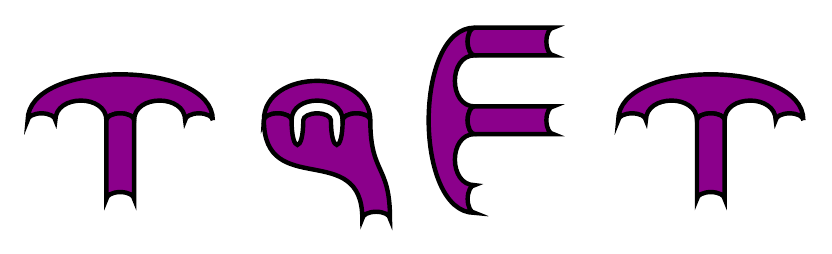
\begin{tikzpicture}[
    scale=.5,
    every tqft/.style={
      transform shape
    },
    tqft/cobordism/.style={
      fill=DarkMagenta,
      draw,
      ultra thick},
  ]
  \pic[
    name=a,
    tqft,
    incoming boundary components=0,
    outgoing boundary components=3,
  ];
  \pic[
    name=b,
    at=(a-outgoing boundary 2),
    tqft cylinder,
    anchor=incoming boundary 1,
  ];
  \pic[
    at=(a-outgoing boundary 3),
    name=c,
    tqft,
    incoming boundary components=0,
    outgoing boundary components=2,
    anchor={(0,1)},
  ];
  \pic[
    at=(c-outgoing boundary 1),
    name=d,
    tqft,
    incoming boundary components=3,
    outgoing boundary components=1,
    offset=2.5,
    anchor=incoming boundary 1,
    boundary separation=1cm,
    cobordism height=2.5cm,
  ];
  \pic[
    at=(c-outgoing boundary 2),
    name=e,
    tqft,
    rotate=90,
    incoming boundary components=0,
    outgoing boundary components=3,
    anchor={(2,-.5)}
  ];
  \pic[
    at=(e-outgoing boundary 3),
    name=f,
    tqft cylinder,
    rotate=90,
    anchor=incoming boundary 1,
  ];
  \pic[
    at=(e-outgoing boundary 2),
    name=g,
    tqft cylinder,
    rotate=90,
    anchor=incoming boundary 1,
  ];
  \pic[
    at=(g-outgoing boundary 1),
    name=h,
    tqft,
    anchor={(0,1)},
    incoming boundary components=0,
    outgoing boundary components=3,
  ];
  \pic[
    at=(h-outgoing boundary 2),
    name=i,
    tqft cylinder,
    anchor=incoming boundary 1,
  ];
\end{tikzpicture}
\end{center}

\section{Introduction}
This package defines some Ti\emph{k}Z/PGF picture shapes that can be used to construct the diagrams common in Topological Quantum Field Theory (TQFT).
An example follows:

\begin{example}
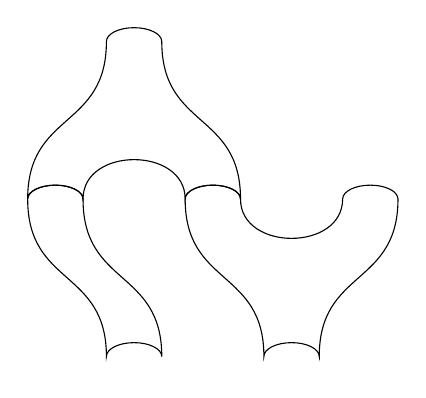
\begin{tikzpicture}[tqft/cobordism/.style={draw}]
\pic[tqft/pair of pants,name=a];
\pic[tqft/cylinder to next,anchor=incoming boundary 1,name=c,at=(a-outgoing boundary 1)];
\pic[tqft/reverse pair of pants, anchor=incoming boundary 1,at=(a-outgoing boundary 2)];
\end{tikzpicture}
\end{example}

\tableofcontents

\section{History}

This is the second version of the TQFT package.
The first version used nodes to draw the shapes.
However, with the advent of Ti\emph{k}Z3.0 came the ability to define subdrawings called \Verb+pic+s which were a bit like nodes but were geared more towards drawings than containers for text.
This seems a much more suitable mechanism for drawing these diagrams and so the package has been rewritten to make use of this new facility.

The second version is designed to be similar to the first, but with some improvements.
The original version was distributed as a \Verb+.sty+ file and so is loaded using \Verb+\usepackage{tqft}+.
The newer version is a Ti\emph{k}Z library and so is loaded using \Verb+\usetikzlibrary{tqft}+.
This makes it possible to use both in the same document.
This is not recommended, but an attempt has been made to make it possible to switch between the two methods (mainly to stop this documentation file complaining every time I compile it).
This hasn't been extensively tested so use with caution.
To make the switch use the key \Verb+/tikz/tqft/use nodes=<true|false>+.
By default, the one loaded last should be in effect at the start of the document.

\section{Keys}

Before giving any details, a word is in order about the keys involved in this package.
There are many options and keys that can be set via the \Verb+\pgfkeys+ system (which is used for setting options in Ti\emph{k}Z).
Such keys live in a ``directory'' but often that can be omitted.
For example, in the Ti\emph{k}Z command \Verb+\draw[red] (0,0) -- (1,0);+ the key \Verb+red+ is actually in the ``directory'' \Verb+/tikz+ but it is not necessary to specify that as it is assumed.
Defining a ``directory'' helps separate keys and ensure that there is no conflict.
The keys in this library are (mostly) defined in the directories \Verb+/tikz/tqft+ (the newer version) and \Verb+/pgf/tqft+ (the old version).

Invoking \Verb+/tikz/tqft+ itself sets the ``current directory'' to whichever directory is right for the current version in force and so all subsequent keys do not need prefixing.
Moreover, any unknown keys are passed on to the \Verb+/tikz+ directory so there is (or should be!) no harm in mixing \Verb+tqft+ specific keys with ordinary Ti\emph{k}Z keys.
Some examples take advantage of this switch so when copying and modifying examples from this document, it is important to remember that the first \Verb+tqft+ specific key needs an explicit \Verb+tqft/+ prefix.


\section{Version 2: Pics via a TikZ Library}
\label{sec:pic}

\subsection{The Shapes}

There is only one picture shape: \Verb+cobordism+.
This is a cobordism between a number of incoming circles and a number of outgoing circles, where the numbers of boundary components can be specified as options to the shape.
There are certain common shapes that are predefined as aliases to the main shape with specified boundaries.
The list of predefined shapes follows.
The names are all in the \Verb+tqft+ family, but an alias is made so that \Verb+tqft <shape>+ will work without any further qualification.

\begin{enumerate}
\item \Verb+pair of pants+

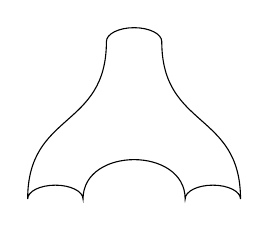
\begin{tikzpicture}
\pic[draw,tqft/pair of pants];
\end{tikzpicture}

\item \Verb+reverse pair of pants+

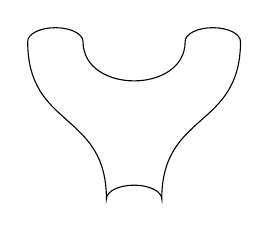
\begin{tikzpicture}
\pic[draw,tqft/reverse pair of pants];
\end{tikzpicture}

\item \Verb+cylinder to prior+

This is a cylinder that has been skewed to one side, thus following the same path as the \Verb+pair of pants+ cobordism but with only one outgoing boundary component.
The name \Verb+to prior+ is because it goes towards the lower-numbered component on the \Verb+pair of pants+. 

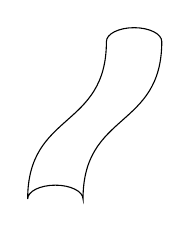
\begin{tikzpicture}
\pic[draw,tqft/cylinder to prior];
\end{tikzpicture}

\item \Verb+cylinder to next+

This is a cylinder that has been skewed to one side, thus following the same path as the \Verb+pair of pants+ cobordism but with only one outgoing boundary component.
The name \Verb+to next+ is because it goes towards the higher-numbered component on the \Verb+pair of pants+. 

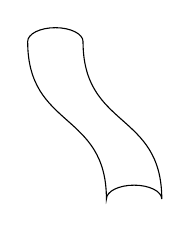
\begin{tikzpicture}
\pic[draw,tqft/cylinder to next];
\end{tikzpicture}

\item \Verb+cylinder+

This is a straight cylinder.

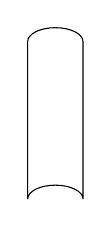
\begin{tikzpicture}
\pic[draw,tqft/cylinder];
\end{tikzpicture}

\item \Verb+cap+

This is a cap.

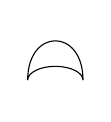
\begin{tikzpicture}
\pic[draw,tqft/cap];
\end{tikzpicture}

\item \Verb+cup+

This is a cup (an upside-down cap).

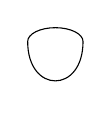
\begin{tikzpicture}
\pic[draw,tqft/cup];
\end{tikzpicture}

\end{enumerate}

The general shape is controlled by the following keys:

\begin{itemize}
\item \DescribeMacro{view from} To get a simulated 3D effect, the cobordism is drawn as if viewed from a slight angle.
The value of this key determines whether the cobordism is viewed from the direction of the incoming boundary components or the outgoing ones.
This key can take the values \Verb+incoming+ and \Verb+outgoing+.
The default is \Verb+outgoing+.
\item \DescribeMacro{cobordism height} This is the height of the cobordism (``height'' interpreted in its own internal coordinate system).
With no offset (q.v.), this would be the distance between the centres of the first incoming and first outgoing boundary components.

\item \DescribeMacro{boundary separation} This is the distance between the centres of the boundary components of the same type.

\item \DescribeMacro{circle x radius} This is the half-width of the boundary circles.

\item \DescribeMacro{circle y radius} This is the half-depth of the boundary circles (``depth'' since, in the internal coordinate system, this corresponds to the \(z\)-axis out of the page).

\item \DescribeMacro{incoming boundary components} The number of incoming boundary components (can be zero).

\item \DescribeMacro{skip incoming boundary components} A list of incoming boundary components to be skipped.

\item \DescribeMacro{outgoing boundary components} The number of outgoing boundary components (can be zero).

\item \DescribeMacro{skip outgoing boundary components} A list of outgoing boundary components to be skipped.

\item \DescribeMacro{offset} This offsets the first outgoing boundary component horizontally relative to the first incoming boundary component.
It is a dimensionless number (not necessarily an integer) and is interpreted so that a value of \(1\) aligns the first outgoing boundary component with the second incoming boundary component.

\item \DescribeMacro{genus} This defines the number of holes in the shape.
These are spread out in a horizontal line in the middle of the shape.

\item \DescribeMacro{twisted} This is a boolean that, if set, makes the cobordism \emph{twisted} in that the edges cross as they pass from the incoming to outgoing boundaries.
This probably won't look good with a non-zero genus, but there's nothing stopping you doing it.
\end{itemize}

\subsection{Styling}

There are various options for styling the diagrams.
To understand how they work, it is important to know the order in which a cobordism is drawn and how many pieces it decomposes into.
This is the following list, with the corresponding keys:

\begin{enumerate}
\item The boundary circles are drawn.
These are actually elliptical nodes (and thus can be individually styled).
Applicable styles:

\begin{itemize}
\item \Verb+every boundary component+,
\item \Verb+every incoming boundary component+,\\
or  \Verb+every outgoing boundary component+,
\item \Verb+incoming boundary component <n>+,\\
or \Verb+outgoing boundary component <n>+
\end{itemize}

\item The lower edges of the boundary circles are redrawn.
These are individual arcs.

\begin{itemize}
\item \Verb+every lower boundary component+,
\item \Verb+every incoming lower boundary component+,\\or  \Verb+every outgoing lower boundary component+,
\item \Verb+incoming lower boundary component <n>+,\\or \Verb+outgoing lower boundary component <n>+
\end{itemize}

\item The full edge of the cobordism is drawn.
This is a closed path so can be sensibly filled.
It is clipped against a path defined by the genus of the cobordism which results in holes if it is filled (or shaded or anything else that goes in to the interior).

\begin{itemize}
\item \Verb+cobordism+,
\item also, any actions specified on the \Verb+pic+ are applied here (specifically, the \Verb+pic actions+ key is invoked; see the Ti\emph{k}Z manual for full details on this),
\item \Verb+cobordism outer path+.
\end{itemize}

\item Any holes specified by the genus are now drawn.
These are styled to give the 3D impression, and this follows the direction specified by the \Verb+view from+ key.
The paths are split so that each can be individually styled.

\begin{itemize}
\item \Verb+cobordism+, this style is applied because the curves defined by the genus can be thought of as part of the edge of the cobordism shape.
\item \Verb+pic actions+, for the same reason as above.

However, following this key then \Verb+fill=none,shade=none+ is issued.
This is because even if the main shape is filled or shaded, the paths drawing the holes should almost certainly not be.
\item \Verb+cobordism edge+, the same logic applies to the edge path (q.v.).
\item \Verb+genus style+,
\item \Verb+genus upper+ or \Verb+genus lower+,
\item \Verb+hole <n>+,
\item \Verb+hole <n> upper+ or \Verb+hole <n> lower+.
\end{itemize}

\item The non-boundary edge of the cobordism is redrawn.
This is split in to pieces to allow for individual styling.

\begin{itemize}
\item \Verb+cobordism edge+,
\item \Verb+cobordism outer edge+,
\item \Verb+between incoming+, or \Verb+between outgoing+, or \Verb+between incoming and outgoing+.
The latter is for the two sides, but note that if the cobordism has no incoming or no outgoing components then it also applies to the ``over the top'' edge.
\item \Verb+<anchor>+, where the \Verb+<anchor>+ is the name of the anchor that lies on the midpoint of the curve, so it will be one of:
%
\begin{itemize}
\item \Verb=between incoming <n> and <n+1>=,
\item \Verb=between outgoing <n> and <n+1>=,
\item \Verb+between first incoming and first outgoing+,
\item \Verb+between last incoming and last outgoing+,
\item \Verb+between first and last incoming+,
\item \Verb+between first and last outgoing+.
\end{itemize}
\end{itemize}

\item The upper edges of the boundary circles are redrawn.
These are arcs.

\begin{itemize}
\item \Verb+every upper boundary component+,
\item \Verb+every incoming upper boundary component+,\\or  \Verb+every outgoing upper boundary component+,
\item \Verb+incoming upper boundary component <n>+,\\or \Verb+outgoing upper boundary component <n>+
\end{itemize}
\end{enumerate}

The fact that there are so many is to allow different style to be applied to different pieces and to give as much control as possible, whilst still making it fairly straightforward to draw a simple cobordism.
The duplication of paths is to allow certain composite pieces to be \emph{filled}.
Here is a progressively built up cobordism.

\begin{example}
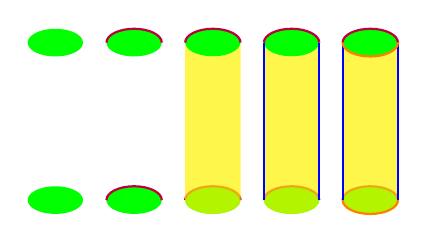
\begin{tikzpicture}[tqft/view from=incoming]
\begin{scope}[tqft/every boundary component/.style={fill=green,fill opacity=1}]
\pic[tqft/cylinder,at={(1,0)}];
\begin{scope}[tqft/every lower boundary component/.style={draw=purple,thick}]
\pic[tqft/cylinder,at={(2,0)}];
\begin{scope}[tqft/cobordism/.style={fill=yellow,fill opacity=.7}]
\pic[tqft/cylinder,at={(3,0)}];
\begin{scope}[tqft/cobordism edge/.style={draw,thick,blue}]
\pic[tqft/cylinder,fill=yellow,fill opacity=.7,at={(4,0)}];
\begin{scope}[tqft/every upper boundary component/.style={draw,thick,orange}]
\pic[tqft/cylinder,fill=yellow,fill opacity=.7,at={(5,0)}];
\end{scope}
\end{scope}
\end{scope}
\end{scope}
\end{scope}
\end{tikzpicture}
\end{example}

Here's an example with lots of styling.

\begin{example}
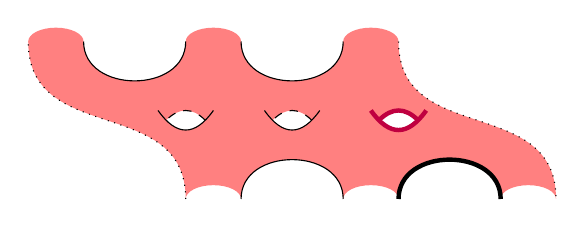
\begin{tikzpicture}
\pic[
  tqft,
  incoming boundary components=3,
  outgoing boundary components=3,
  offset=1,
  genus=3,
  hole 3/.style={ultra thick, purple,solid},
  genus lower/.style={dashed},
  fill=red!50,
  cobordism edge/.style={draw},
  between incoming and outgoing/.style={dotted},
  between outgoing 2 and 3/.style={ultra thick},
];
\end{tikzpicture}
\end{example}

\subsection{Anchors}

The cobordism is a \Verb+pic+ so does not have any native anchors.
Nevertheless, a multitude of coordinates are defined that simulate the anchors associated with nodes.
There is also support for specifying the shape to be located relative to a particular anchor.

The \Verb+\pic+ should be named via the \Verb+name=<prefix>+ key, whereupon the anchors are prefixed by this value.
The pseudo-anchors defined have the naming convention \Verb+<prefix>-<anchor name>+ (at the moment, it doesn't check to see if the \Verb+name+ key has been specified so if it isn't then the pseudo-anchors are still defined but with an empty prefix).
They are:
%
\begin{itemize}
\item \Verb+incoming boundary <n>+, these are in fact elliptical nodes and so also define actual anchors.
\item \Verb+incoming boundary+ is an alias for \Verb+incoming boundary 1+.
\item \Verb+outgoing boundary <n>+, same.
\item \Verb+outgoing boundary+ is an alias for \Verb+outgoing boundary 1+.
\item \Verb=between incoming <n> and <n+1>=, this lies on the midpoint of the curve between successive boundary components.
\item \Verb=between outgoing <n> and <n+1>=, this lies on the midpoint of the curve between successive boundary components.
\item \Verb=between first incoming and first outgoing= is on the edge between the first incoming and first outgoing boundary components; note that this is only defined if there are both incoming and outgoing boundary components.
\item \Verb=between last incoming and last outgoing= is on the edge between the last incoming and last outgoing boundary components; note that this is only defined if there are both incoming and outgoing boundary components.
\item \Verb=between first and last incoming=; this is only defined if there are no outgoing components.

This is also available via the alias \Verb=between first incoming and last incoming=.
\item \Verb=between first and last outgoing=; this is only defined if there are no incoming components.

This is also available via the alias \Verb=between first outgoing and last outgoing=.
\item \Verb=hole <n>=; if the genus is non-zero, this points to the centre of the \(n\)th hole.
\end{itemize}

To place the shape relative to an anchor, use the \Verb+tqft/anchor+ key.
The argument should be just the name of the anchor without the leading \Verb+<prefix>-+.
The \Verb+anchor+ key can also take another type of argument.
If its argument is of the form \Verb+(x,y)+ then this is taken as a pseudo-coordinate\footnote{Note that due to the presence of the comma, this type of argument must be protected by braces.}.
It is interpreted as being \(x\) boundary components across and \(y\) times the cobordism height down.
However, if an \Verb+offset+ is specified then the resulting \(x\) value is shifted so that if \(y < 0\) then \((1,y)\) is in line with the first incoming boundary component and if \(y > 1\) then \((1,y)\) is in line with the first outgoing boundary component.
If \(0 < y < 1\) then \((1,y)\) linearly interpolates between the first incoming and first outgoing boundary components.
Thus \((1,0)\) is the first incoming boundary component, \((1,1)\) the first outgoing boundary component, \((0,0)\) is one unit to the left of the first incoming, and \((1,2)\) one unit below the first outgoing.
Note that the picture is shifted to put this point at the current coordinate.

\begin{example}
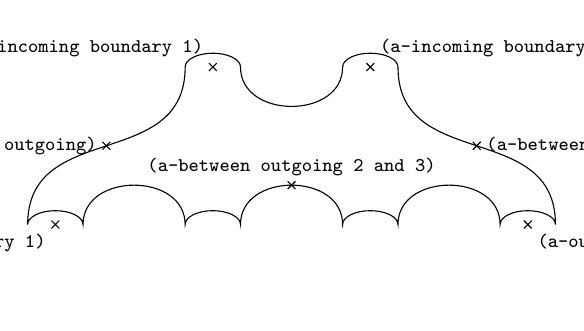
\begin{tikzpicture}
\pic[tqft, incoming boundary components=2,outgoing boundary components=4,offset=-1,draw,name=a];
\foreach \anchor/\placement in
{
between first incoming and first outgoing/left,
between last incoming and last outgoing/right,
between outgoing 2 and 3/above,
incoming boundary 1/above left,
incoming boundary 2/above right,
outgoing boundary 1/below left,
outgoing boundary 4/below right}
\draw[overlay,shift=(a-\anchor)] plot[mark=x] coordinates{(0,0)} node[\placement] {\scriptsize\texttt{(a-\anchor)}};
\path (a-incoming boundary) +(0,.5) (a-outgoing boundary) +(0,-1);
\end{tikzpicture}
\end{example}

\subsection{Notes}

\begin{enumerate}
\item Like \Verb+node+s, \Verb+pic+s need the \Verb+transform shape+ key to be set to take note of external transformations (other than shifts).
The tqft pic uses nodes internally and those nodes have \Verb+transform shape+ automatically set so this should \emph{just work}.
\item There is an additional \Verb+every tqft+ key which is run when the \Verb+tqft+ key is invoked (which might be via some other key).
This is better placed than the \Verb+every pic+ key since that applies to a surrounding scope rather than to the \Verb+pic+ itself.
\item If the \Verb+tqft+ key is invoked, either implicitly or explicitly, then the \Verb+pic type+ is set to \Verb+cobordism+.
This has the side effect that the invoking syntax has to be completely set by keys; so the \Verb+pic (<name>) at (<coord>) {<type>}+ cannot be used.
Rather, the \Verb+name+ and \Verb+at+ have to be specified by keys and the \Verb+type+ omitted.

\item If upgrading from the previous version of TQFT, as well as shifting from a \Verb+node+ to a \Verb+pic+, the following changes have been made in the implementation:

\begin{itemize}
\item The \Verb+flow+ key has not made it across to the new version.
Use \Verb+transform shape+ and apply your own transformation.

\item The \Verb+circle width+ and \Verb+circle depth+ are now \Verb+circle x radius+ and \Verb+circle y radius+ (the old names weren't correct anyway).

\item The bounding box is a little better, particularly for cobordisms with only one type of boundary component.
\end{itemize}
\end{enumerate}

\subsection{More Examples}

\begin{example}
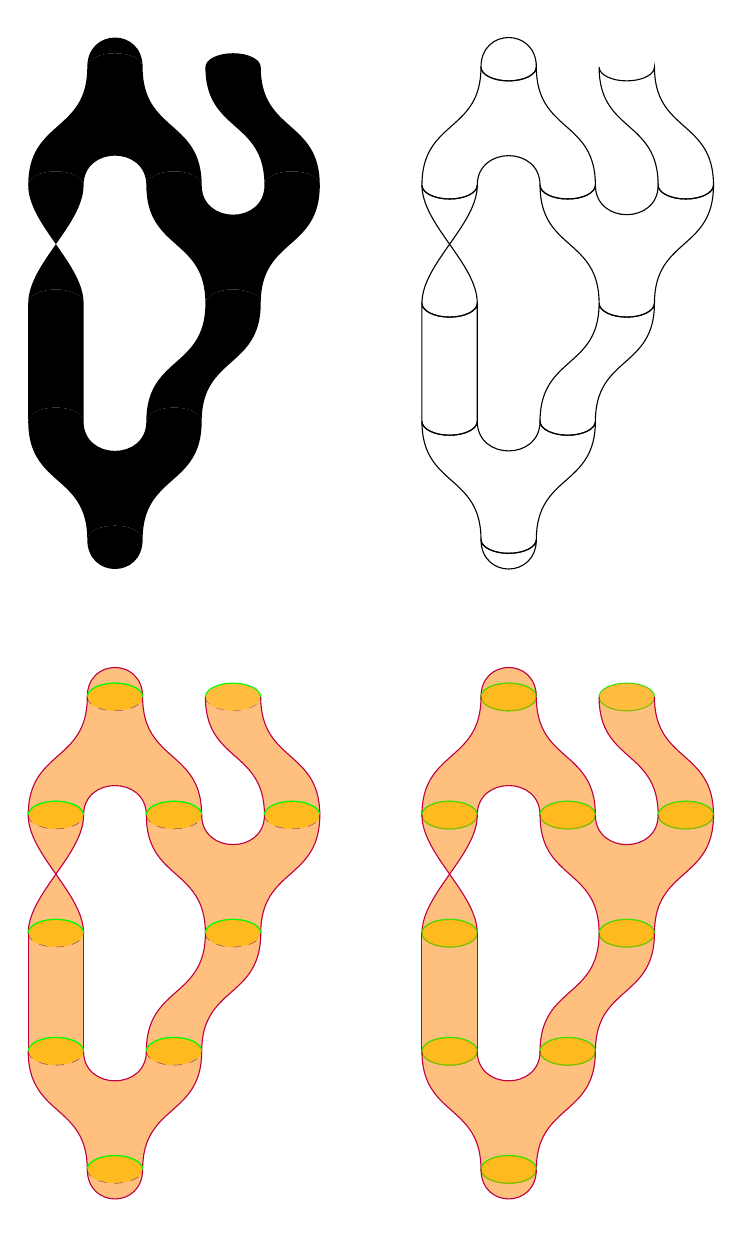
\begin{tikzpicture}[tqft/cobordism height=1.5cm,tqft/boundary  separation=1.5cm]
\foreach \coord/\style in {
{(0,0)}/{tqft/view from=outgoing,fill},
{(5,0)}/{tqft/view from=incoming,draw},
{(0,-8)}/{fill=orange,fill opacity=.5,tqft/every lower boundary component/.style={draw,blue,ultra thin,dashed},tqft/every upper boundary component/.style={draw,green},tqft/cobordism edge/.style={draw,purple},tqft/every boundary component/.style={fill=yellow}},
{(5,-8)}/{fill=orange,fill opacity=.5,tqft/cobordism edge/.style={draw,purple},tqft/every boundary component/.style={fill=yellow,draw=green}}
} {
  \begin{scope}[every tqft/.style/.expand once=\style]
\pic[tqft/cap,name=h,at=\coord];
\pic[tqft/pair of pants,anchor=incoming boundary 1,name=a,at=(h-outgoing boundary 1)];
\pic[tqft/cylinder to next,anchor={(0,1)},name=d,at=(a-outgoing boundary 2)];
\pic[tqft/reverse pair of pants,anchor=incoming boundary 1,name=b,at=(a-outgoing boundary 2)];
\pic[tqft/cylinder to prior,anchor=incoming boundary 1,name=c,at=(b-outgoing boundary 1)];
\pic[tqft/cylinder,twisted,anchor=incoming boundary 1,name=e,at=(a-outgoing  boundary 1)];
\pic[tqft/cylinder,anchor=incoming boundary 1,name=f,at=(e-outgoing  boundary 1)];
\pic[tqft/reverse pair of pants,anchor=incoming boundary 1,name=g,at=(f-outgoing boundary 1)];
\pic[tqft/cup,anchor=incoming boundary 1,name=i,at=(g-outgoing boundary 1)];
\end{scope}
}
\end{tikzpicture}
\end{example}

\begin{example}
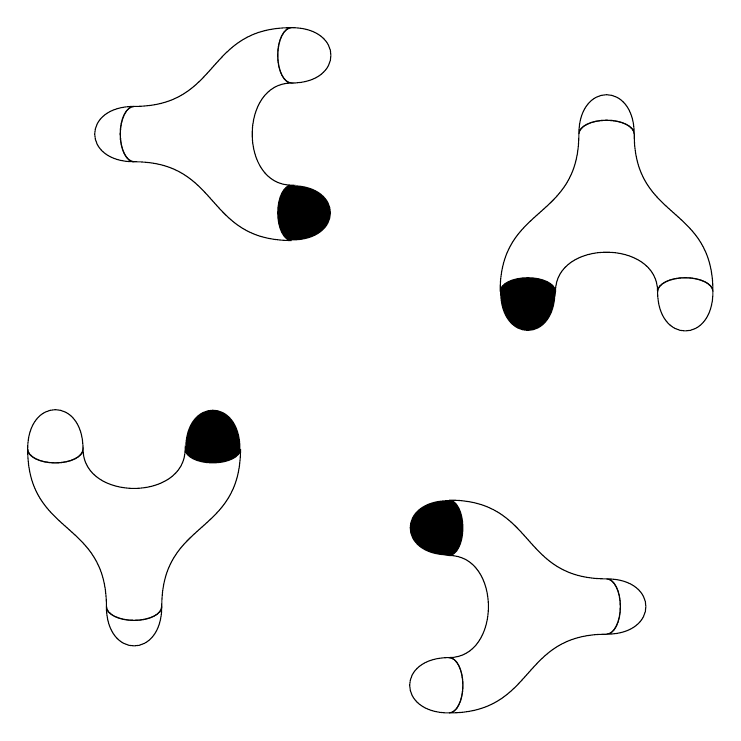
\begin{tikzpicture}[every tqft/.append style={transform shape}]
\foreach \ang in {0,90,180,270} {
\begin{scope}[rotate=\ang]
\pic[draw,tqft/pair of pants,name=a,at={(3,3)}];
\pic[draw,tqft/cap,anchor=outgoing boundary 1,at=(a-incoming boundary 1)];
\pic[fill,tqft/cup,anchor=incoming boundary 1,at=(a-outgoing boundary 1)];
\pic[draw,tqft/cup,anchor=incoming boundary 1,at=(a-outgoing boundary 2)];
\end{scope}
}
\end{tikzpicture}
\end{example}

\begin{example}
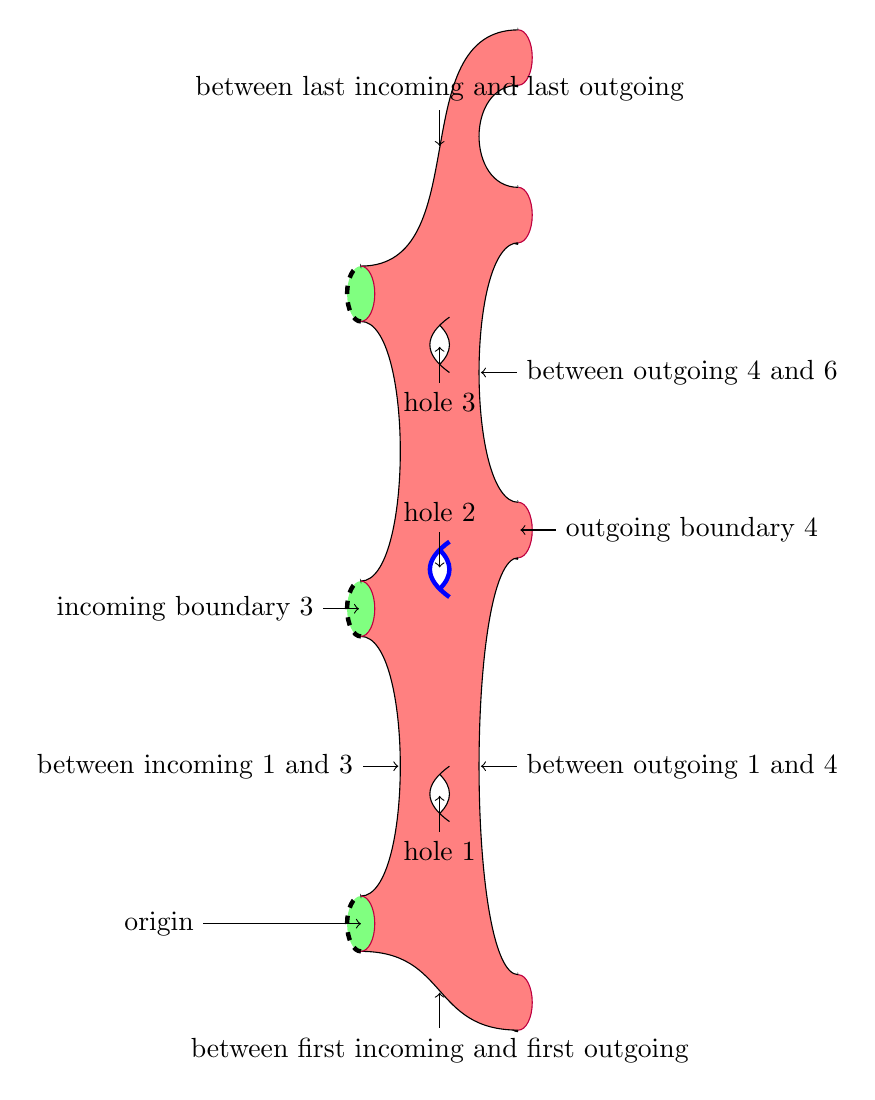
\begin{tikzpicture}[
  tqft,
  every outgoing boundary component/.style={fill=blue!50},
  outgoing boundary component 3/.style={fill=none,draw=red},
  every incoming boundary component/.style={fill=green!50},
  every lower boundary component/.style={draw,ultra thick, dashed},
  every upper boundary component/.style={draw,purple},
  cobordism/.style={fill=red!50},
  cobordism edge/.style={draw},
  genus=3,
  hole 2/.style={ultra thick, blue},
  view from=incoming,
  anchor=between incoming 1 and 2
]
\pic[rotate=90,
  %every node/.style={transform shape},
  name=a,tqft,incoming boundary components=5,skip incoming boundary components={2,4},outgoing boundary components=7,skip outgoing boundary components={2,3,5},offset=-.5];

\begin{scope}[every pin edge/.style={<-}]
\foreach \anchor/\ang in {
  hole 1/-90,
  hole 2/90,
  hole 3/-90,
  incoming boundary 3/180,
  outgoing boundary 4/0,
  between last incoming and last outgoing/90,
  between first incoming and first outgoing/-90,
  between incoming 1 and 3/180,
  between outgoing 1 and 4/0,
  between outgoing 4 and 6/0
} {
  \node[pin=\ang:\anchor,at=(a-\anchor),inner sep=0pt] {};
}
\draw[<-] (0,0) -- ++(-2,0) node[left] {origin};
\end{scope}
\end{tikzpicture}
\end{example}

%\begin{example}
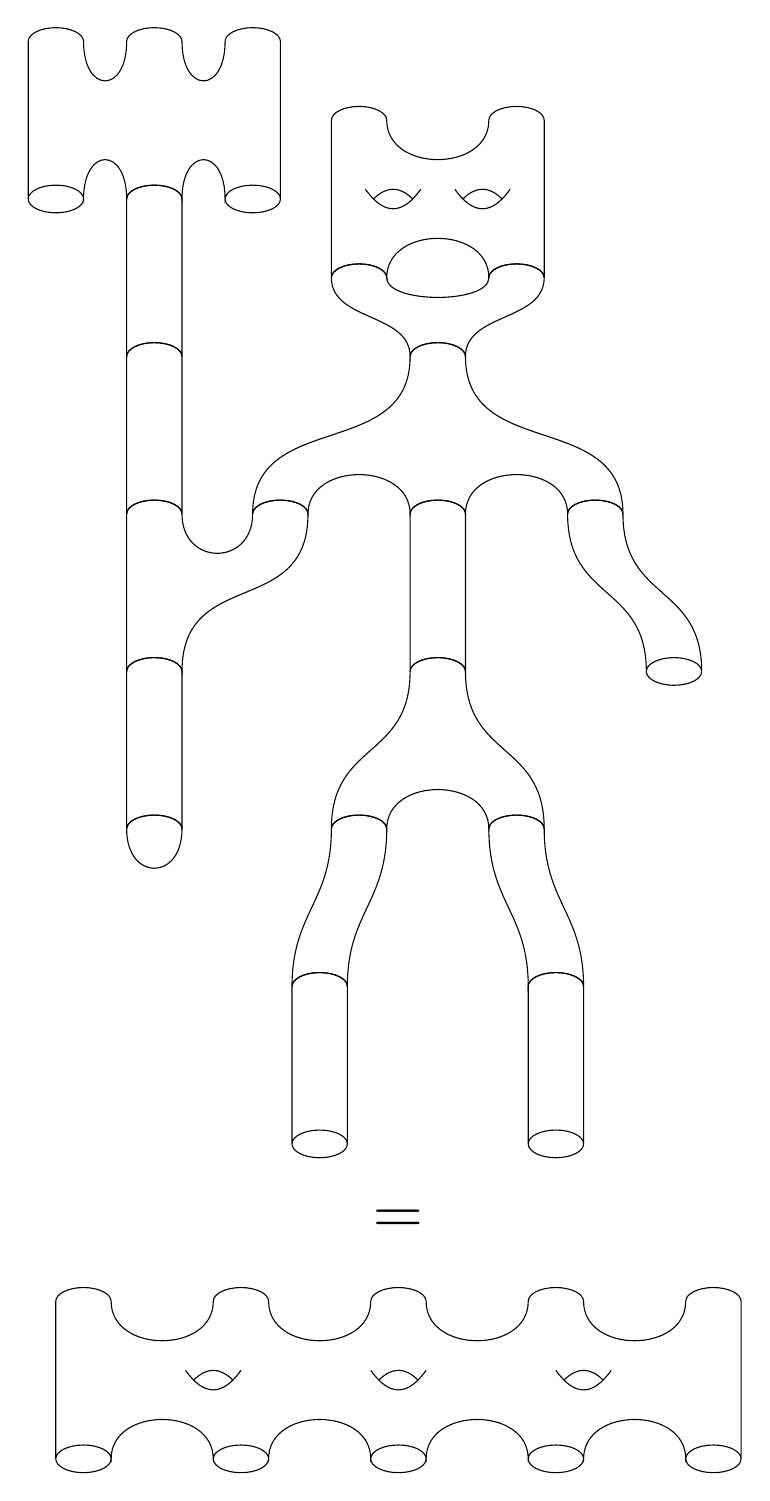
\begin{tikzpicture}
\pic[
  tqft,
  incoming boundary components=2,
  outgoing boundary components=2,
  genus=2,
  draw,
  name=a
];
\pic[
  tqft,
  incoming boundary components=2,
  outgoing boundary components=1,
  draw,
  at=(a-outgoing boundary 1),
  offset=.5,
  cobordism height=1cm,
  name=b
];
\pic[tqft,
  incoming boundary components=1,
  outgoing boundary components=3,
  draw,
  at=(b-outgoing boundary 1),
  offset=-1,
  name=c
];
\pic[tqft,
  incoming boundary components=2,
  outgoing boundary components=1,
  draw,
  at=(c-outgoing boundary 1),
  anchor=incoming boundary 2,
  name=d,
  boundary separation=1.6cm,
];
\pic[tqft,
  incoming boundary components=1,
  outgoing boundary components=1,
  draw,
  at=(c-outgoing boundary 3),
  offset=.5,
  name=e,
  every outgoing lower boundary component/.style={draw}
];
\pic[tqft,
  incoming boundary components=1,
  outgoing boundary components=1,
  draw,
  at=(c-outgoing boundary 2),
  name=f
];
\pic[tqft,
  incoming boundary components=1,
  outgoing boundary components=2,
  draw,
  at=(f-outgoing boundary),
  name=g,
  offset=-.5,
];
\pic[tqft,
  incoming boundary components=1,
  outgoing boundary components=1,
  draw,
  at=(g-outgoing boundary 1),
  name=h,
  offset=-.25,
];
\pic[tqft,
  incoming boundary components=1,
  outgoing boundary components=1,
  draw,
  at=(g-outgoing boundary 2),
  name=i,
  offset=.25,
];
\pic[tqft,
  incoming boundary components=1,
  outgoing boundary components=1,
  draw,
  at=(h-outgoing boundary),
  name=j,
  every outgoing lower boundary component/.style={draw}
];
\pic[tqft,
  incoming boundary components=1,
  outgoing boundary components=1,
  draw,
  at=(i-outgoing boundary),
  name=k,
  every outgoing lower boundary component/.style={draw}
];
\pic[tqft,
  incoming boundary components=1,
  outgoing boundary components=1,
  draw,
  at=(d-outgoing boundary),
  name=l
];
\pic[tqft,
  incoming boundary components=1,
  outgoing boundary components=0,
  draw,
  at=(l-outgoing boundary),
  name=m
];
\pic[tqft,
  incoming boundary components=1,
  outgoing boundary components=1,
  draw,
  at=(d-incoming boundary),
  anchor=outgoing boundary,
  name=n
];
\pic[tqft,
  incoming boundary components=1,
  outgoing boundary components=1,
  draw,
  at=(n-incoming boundary),
  anchor=outgoing boundary,
  name=o
];
\pic[tqft,
  incoming boundary components=3,
  outgoing boundary components=3,
  draw,
  at=(o-incoming boundary),
  anchor={(2,1)},
  name=p,
  boundary separation=1.25cm,
  outgoing lower boundary component 1/.style={draw},
  outgoing lower boundary component 3/.style={draw}
];
\pic[tqft,
  incoming boundary components=5,
  outgoing boundary components=5,
  genus=3,
  at=(k-outgoing boundary),
  anchor={(4,-1)},
  draw,
  name=q,
  every outgoing lower boundary component/.style={draw}
];
\path (q-incoming boundary 3) ++(0,1) node {\Huge \(=\)};
\end{tikzpicture}
%\end{example}

\section{Version 1: Nodes via a Style File}

\tikzset{tqft/use nodes=true}

As mentioned in the introduction, this is the original method of drawing cobordism diagrams using nodes and is no longer updated (though I will fix bugs if I can).
If drawing a new diagram, use the pic method from Section~\ref{sec:pic}.

\subsection{The Node Shapes}

There are only two shapes, \Verb+tqft cobordism+ and \Verb+tqft boundary circle+.
The first, which is the main shape, is a cobordism between a number of incoming circles and a number of outgoing circles, where the numbers of boundary components can be specified as options to the shape.
The second is just the boundary circle.
It is used as a sub-node of the first to add extra anchors, but can be used by itself.
There are certain common shapes that are predefined as aliases to the main shape with specified boundaries.
The list of predefined shapes follows.
The names are all in the \Verb+tqft+ family, but an alias is made so that \Verb+tqft nodeshape+ will work without any further qualification.

\begin{enumerate}
\item \Verb+pair of pants+

\begin{tikzpicture}
\node[draw,tqft/pair of pants] (a) {};
\end{tikzpicture}

\item \Verb+reverse pair of pants+

\begin{tikzpicture}
\node[draw,tqft/reverse pair of pants] (a) {};
\end{tikzpicture}

\item \Verb+cylinder to prior+

This is a cylinder that has been skewed to one side, thus following the same path as the \Verb+pair of pants+ cobordism but with only one outgoing boundary component.
The name \Verb+to prior+ is because it goes towards the lower-numbered component on the \Verb+pair of pants+. 

\begin{tikzpicture}
\node[draw,tqft/cylinder to prior] (a) {};
\end{tikzpicture}

\item \Verb+cylinder to next+

This is a cylinder that has been skewed to one side, thus following the same path as the \Verb+pair of pants+ cobordism but with only one outgoing boundary component.
The name \Verb+to next+ is because it goes towards the higher-numbered component on the \Verb+pair of pants+. 

\begin{tikzpicture}
\node[draw,tqft/cylinder to next] (a) {};
\end{tikzpicture}

\item \Verb+cylinder+

This is a straight cylinder.

\begin{tikzpicture}
\node[draw,tqft/cylinder] (a) {};
\end{tikzpicture}

\item \Verb+cap+

This is a cap.

\begin{tikzpicture}
\node[draw,tqft/cap] (a) {};
\end{tikzpicture}

\item \Verb+cup+

This is a cup (an upside-down cap).

\begin{tikzpicture}
\node[draw,tqft/cup] (a) {};
\end{tikzpicture}

\end{enumerate}

The general shape is controlled by the following keys:

\begin{itemize}
\item \DescribeMacro{flow} A cobordism ``flows'' from its incoming to its outgoing boundaries.
This key controls the direction of that flow.
The shape is transformed so that the incoming-outgoing axis aligns with the argument.
However, the transformation may be more than just a rotation as the shape is set up so that the numbering of the boundary components is always left-to-right or top-to-bottom (as appropriate).
Currently, this key can take the values \Verb+north+, \Verb+south+ (default), \Verb+east+, and \Verb+west+.

\item \DescribeMacro{view from} To get a simulated 3D effect, the cobordism is drawn as if viewed from a slight angle.
The value of this key determines whether the cobordism is viewed from the direction of the incoming boundary components or the outgoing ones.
This key can take the values \Verb+incoming+ and \Verb+outgoing+.
The default is \Verb+outgoing+.
\item \DescribeMacro{cobordism height} This is the height of the cobordism (``height'' interpreted in its own internal coordinate system).
With no offset (q.v.), this would be the distance between the centres of the first incoming and first outgoing boundary components.

\item \DescribeMacro{boundary separation} This is the distance between the centres of the boundary components of the same type.

\item \DescribeMacro{circle width} This is the half-width of the boundary circles.

\item \DescribeMacro{circle depth} This is the half-depth of the boundary circles (``depth'' since, in the internal coordinate system, this corresponds to the \(z\)-axis out of the page).

\item \DescribeMacro{incoming boundary components} The number of incoming boundary components (can be zero).

\item \DescribeMacro{outgoing boundary components} The number of outgoing boundary components (can be zero).

\item \DescribeMacro{offset} This offsets the first outgoing boundary component horizontally relative to the first incoming boundary component.
It is a dimensionless number (not necessarily an integer) and is interpreted so that a value of \(1\) aligns the first outgoing boundary component with the second incoming boundary component.
\end{itemize}

\subsection{Styling}

There are various options for styling the diagrams.
To understand how they work, it is important to know the order in which a cobordism is drawn and how many pieces it decomposes into.
This is the following list, with the corresponding key:

\begin{enumerate}
\item The boundary circles are drawn.
\Verb+boundary style+
\item The lower edges of the boundary circles are redrawn.
\Verb+boundary lower style+
\item The cobordism itself is drawn.
\item The non-boundary edge of the cobordism is redrawn.
\Verb+cobordism style+
\item The upper edges of the boundary circles are redrawn.
\Verb+boundary upper style+
\end{enumerate}

The fact that there are so many is to allow different style to be applied to different pieces.
The duplication is to allow certain composite pieces to be \emph{filled}.
All of these items can be styled separately.
The style given to the node itself is passed on to the third item in that list, the cobordism itself.
The styles of the others are controlled by a series of keys, each of should be a list of styles to be applied to that component.
Not all options make sense, in particular only the first and third can be filled.
(That is, the \Verb+fill+ style is ignored on the other components.)
Here is a progressively built up cobordism.

\begin{example}
\begin{tikzpicture}
\begin{scope}[tqft/boundary style={fill=purple,fill opacity=1}]
\node[tqft/cylinder] at (1,0) {};
\begin{scope}[tqft/boundary lower style={draw,dashed,green,thick}]
\node[tqft/cylinder] at (2,0) {};
\begin{scope}
\node[tqft/cylinder,fill=yellow,fill opacity=.7] at (3,0) {};
\begin{scope}[tqft/cobordism style={draw,thick,blue}]
\node[tqft/cylinder,fill=yellow,fill opacity=.7] at (4,0) {};
\begin{scope}[tqft/boundary upper style={draw,thick,orange}]
\node[tqft/cylinder,fill=yellow,fill opacity=.7] at (5,0) {};
\end{scope}
\end{scope}
\end{scope}
\end{scope}
\end{scope}
\end{tikzpicture}
\end{example}

\subsection{Anchors}

As with all PGF node shapes, there are certain anchors defined by the \Verb+tqft+ shape.
These are the \Verb+center+ (and \Verb+centre+) anchors and the \Verb+incoming boundary n+, \Verb+outgoing boundary n+ anchors.
The positioning of the \Verb+center+ anchor is slightly unusual in that if there are no, say, incoming boundary components then the centre anchor is still at the same height above the outgoing boundary components as if there were incoming boundary components.
The reason for this is two-fold: computing the \emph{actual} centre of the shape in such circumstances would be tricky, and when aligning these shapes it is more useful to have the anchors consistent across shapes of varying boundary components.

There are also the directional anchors \Verb+north+, \Verb+south+, \Verb+east+, \Verb+west+, \Verb+north east+, \Verb+north west+, \Verb+south east+, \Verb+south west+.
The \Verb+east+ and \Verb+west+ anchors are placed at the midpoints of the sides.
The \Verb+north+ and \Verb+south+ anchors are placed in a vertical line with the \Verb+center+ anchor and vertically aligned with the centres of the corresponding boundary circles.
The other four directional anchors are placed at the corners of the cobordism (the placement of these anchors in the case that there are no boundary circles in the corresponding direction may change in future versions).

The \Verb+incoming boundary n+ and \Verb+outgoing boundary n+ are placed at the centres of the corresponding boundary components, with the numbering starting at the left or the top as appropriate to the flow of the cobordism.
A hack borrowed from the \Verb+regular polygon+ shape ensures that there are always enough anchors for the boundary components.

There are also anchors placed at the midpoint of the cobordism edge between the boundary circles.
The names of these are \Verb+after incoming boundary n+ and \Verb+after outgoing boundary n+.

The above anchors can all be ``floated'' off the cobordism using the keys \Verb+outer sep+, \Verb+outer xsep+, and \Verb+outer ysep+.
The last two are the ones actually used, the first is a shortcut for setting both simultaneously.

There are also ``sub-nodes''.
Provding the main node is named, each boundary circle is covered by a \Verb+tqft boundary circle+ node.
This means that the anchors of the \Verb+tqft boundary circle+ can be used.
These cannot be used for placing the main shape, but can be used afterwards.
These are not affected by the \Verb+outer (x/y)sep+ keys.
The names of these sub-nodes are of the form \Verb+name incoming n+ and \Verb+name outgoing n+ where \Verb+name+ is the name of the main node.
The \Verb+tqft boundary circle+ shape is based on an ellipse and defines a boundary so the syntax \Verb+(name.angle)+ works as expected.
It also defines anchors \Verb+next+, \Verb+prior+, \Verb+above+, and \Verb+below+.
These correspond to where the boundary circle in the prescribed direction should be placed.

\begin{example}
\begin{tikzpicture}
\node[tqft, incoming boundary components=2,outgoing boundary components=4,offset=-1,draw] (a) {};
\foreach \anchor/\placement in
{
north/above,
south/below,
east/right,
west/left,
north west/left,
south west/left,
north east/right,
south east/right,
incoming boundary 1/above left,
incoming boundary 2/above right,
outgoing boundary 1/below left,
outgoing boundary 4/below right,
after outgoing boundary 1/below}
\draw[shift=(a.\anchor)] plot[mark=x] coordinates{(0,0)} node[\placement] {\scriptsize\texttt{(a.\anchor)}};
\end{tikzpicture}
\end{example}

\begin{example}
\begin{tikzpicture}
\node[tqft,cylinder, circle width=2cm, circle depth=1cm, cobordism height=4cm,boundary separation=3cm,draw] (b) {};
\foreach \anchor/\placement in
{
prior/left,
next/right,
above/above,
below/below,
0/right,
60/right,
200/left}
\draw[shift=(b incoming 1.\anchor)] plot[mark=x] coordinates{(0,0)} node[\placement] {\scriptsize\texttt{(b incoming 1.\anchor)}};
\end{tikzpicture}
\end{example}

\subsection{Improvements}

Here are some ideas for extending this, and some minor ``bugs''.

\begin{enumerate}
\item Make \Verb+incoming boundary+ an alias of \Verb+incoming boundary 1+ so that if there is only one incoming boundary component then we don't need to specify the number (ditto outgoing).
\item No thought has been given as to where the text gets placed if it is specified.
\item Add the ability to hide certain boundary components.
This is useful if the shapes are not specified in their natural order so certain boundary components should be hidden behind earlier drawn shapes.
\item Some style options on the main node get passed to the other pieces (\Verb+fill opacity+ being one).
This shouldn't happen, or should happen by design not by accident.
\item The bounding box isn't as good as it could be.
\item Add a way to specify more directions for the flow.
\item Add the ability to apply different styles to the incoming and outgoing components.
\end{enumerate}

\subsection{More Examples}

\begin{example}
\begin{tikzpicture}[tqft/cobordism height=1.5cm,tqft/boundary  separation=1.5cm]
\foreach \coord/\style in {
{(0,0)}/{tqft/view from=outgoing,fill},
{(5,0)}/{tqft/view from=incoming,draw},
{(0,-8)}/{fill=orange,fill opacity=.5,tqft/boundary lower  style={draw,blue,ultra thin,dashed},tqft/boundary upper  style={draw,green},tqft/cobordism style={draw,purple},tqft/boundary  style={fill=yellow}},
{(5,-8)}/{fill=orange,fill opacity=.5,tqft/cobordism  style={draw,purple},tqft/boundary style={fill=yellow,draw=green}}
} {
\begin{scope}[every node/.style/.expand once=\style]
\node[tqft/cap] (h) at \coord {};
\node[tqft/pair of pants,anchor=incoming boundary 1] (a) at  (h.outgoing boundary 1) {};
\node[tqft/cylinder to next,anchor=incoming boundary 1] (d) at  (a.incoming boundary 2) {};
\node[tqft/reverse pair of pants,anchor=incoming boundary 1] (b) at (a.outgoing boundary 2) {};
\node[tqft/cylinder to prior,anchor=incoming boundary 1] (c) at  (b.outgoing boundary 1) {};
\node[tqft/cylinder,anchor=incoming boundary 1] (e) at (a.outgoing  boundary 1) {};
\node[tqft/cylinder,anchor=incoming boundary 1] (f) at (e.outgoing  boundary 1) {};
\node[tqft/reverse pair of pants,anchor=incoming boundary 1] (g) at  (f.outgoing boundary 1) {};
\node[tqft/cup,anchor=incoming boundary 1] (i) at (g.outgoing boundary 1) {};
\end{scope}
}
\end{tikzpicture}
\end{example}

\begin{example}
\begin{tikzpicture}
\node[draw,tqft/pair of pants] (a) {};
\node[draw,tqft/cap,anchor=outgoing boundary 1] at (a.incoming boundary 1) {};
\node[fill,tqft/cup,anchor=incoming boundary 1] at (a.outgoing boundary 1) {};
\node[draw,tqft/cup,anchor=incoming boundary 1] at (a.outgoing boundary 2) {};
\begin{scope}[tqft/flow=east]
\node[draw,tqft/pair of pants] (a) at (4,0) {};
\node[draw,tqft/cap,anchor=outgoing boundary 1] at (a.incoming boundary 1) {};
\node[fill,tqft/cup,anchor=incoming boundary 1] at (a.outgoing boundary 1) {};
\node[draw,tqft/cup,anchor=incoming boundary 1] at (a.outgoing boundary 2) {};
\end{scope}
\begin{scope}[tqft/flow=north]
\node[draw,tqft/pair of pants] (a) at (0,-4) {};
\node[draw,tqft/cap,anchor=outgoing boundary 1] at (a.incoming boundary 1) {};
\node[fill,tqft/cup,anchor=incoming boundary 1] at (a.outgoing boundary 1) {};
\node[draw,tqft/cup,anchor=incoming boundary 1] at (a.outgoing boundary 2) {};
\end{scope}
\begin{scope}[tqft/flow=west]
\node[draw,tqft/pair of pants] (a) at (4,-4) {};
\node[draw,tqft/cap,anchor=outgoing boundary 1] at (a.incoming boundary 1) {};
\node[fill,tqft/cup,anchor=incoming boundary 1] at (a.outgoing boundary 1) {};
\node[draw,tqft/cup,anchor=incoming boundary 1] at (a.outgoing boundary 2) {};
\end{scope}
\end{tikzpicture}
\end{example}

\end{document}
